\documentclass[a4paper]{article}

%% Language and font encodings
\usepackage[english]{babel}
\usepackage[utf8x]{inputenc}
\usepackage[T1]{fontenc}

%% Sets page size and margins
\usepackage[a4paper,top=3cm,bottom=2cm,left=3cm,right=3cm,marginparwidth=1.75cm]{geometry}

%% Useful packages
\usepackage{amsmath}
\usepackage{graphicx}
\usepackage[colorinlistoftodos]{todonotes}
\usepackage[colorlinks=true, allcolors=blue]{hyperref}

%% Use Apacite
\usepackage{apacite}

%% For Source code
\usepackage{listings}
\usepackage{color}

\definecolor{dkgreen}{rgb}{0,0.6,0}
\definecolor{gray}{rgb}{0.5,0.5,0.5}
\definecolor{mauve}{rgb}{0.58,0,0.82}

\lstset{frame=tb,
  language=python,
  aboveskip=3mm,
  belowskip=3mm,
  showstringspaces=false,
  columns=flexible,
  basicstyle={\small\ttfamily},
  numbers=none,
  numberstyle=\tiny\color{gray},
  keywordstyle=\color{blue},
  commentstyle=\color{dkgreen},
  stringstyle=\color{mauve},
  breaklines=true,
  breakatwhitespace=true,
  tabsize=3
}

\title{IFT6285 TP}
\author{Jeanne, Jason WU}

\begin{document}
\maketitle

\begin{abstract}
Dans ce travail pratique,  on discutera les methodes de la prédiction d'une séquence de formes à partir d'une séquence de lemmes.
\end{abstract}

\section{Introduction}
What's our purpose?

We are providing the samples with two lines of words, the words linked to a sentence. one line is the word with the tense, another line is the lemma of the word. A lemma is the canonical form of a set of words. For example, 'found, finds, find' are words with tense of the word 'find' as the lemma.

We should implement a system to predict the pattern sequences by dealing with lemma sequences. We may call this issue as 'form-lemma' mapping issue. We are not just focusing on how to find a solution on solving the mapping issue, What we would like to know is how many classifier models we could take into account, and we would choose which one of them to implement our notion. We would also like to know the accuracy of our prediction system for predicting and we should try to improve the accuracy rate with kinds of different methods.

Accuracy = $\frac{true\_positive}{true\_positive + false\_positive}$ = $\frac{\#true\_positive}{\#total\_words}$

\section{Analyst the data}

\subsection{The characteristics of the data}
The data in three sets are contains of English language, they are extracted from wikipedia and is encoded in utf-8. It comes from totally 2020 slices of 1000 articles. The article is represented by a succession of lines, and a line represents a word with the format(form,tab,lemma), each sentence is marked with an empty line. We can get below characteristics according to this information:
\begin{itemize}
\item English language
\item Encoded in utf-8
\item There is connection between words because the words compose a sentence
\item There is a mapping relation between form and lemma
\item Take word as an unit, lemma can be treated as the input, and the form as label
\begin{center}
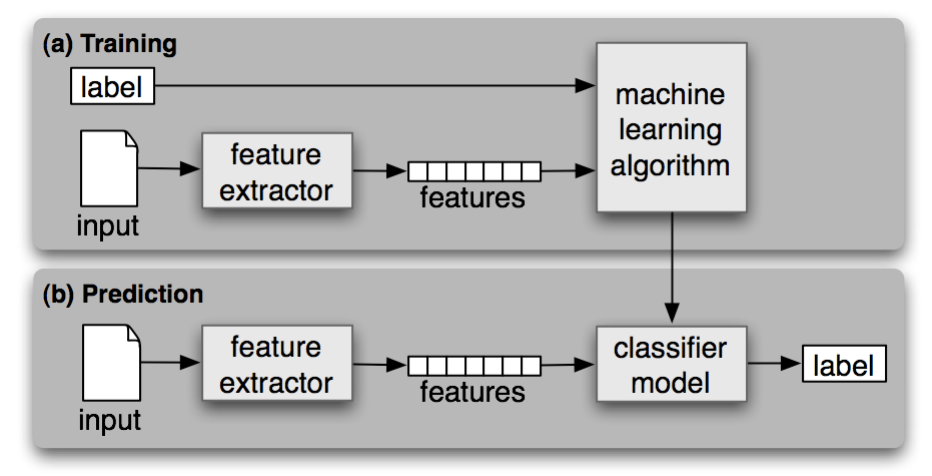
\includegraphics[width=0.8\textwidth]{process_flow.png}
\end{center}
\item Take sentence as a whole object, the sentence which is formed by lemmas and it can be taken as an observation sequence, and the sentence formed by forms as state sequence


\end{itemize}

\subsection{The relation between Training set, Dev-Test Set and Test Set}

We would use the training set to train our feature-based model, Then we can apply our model on dev-test set to optimize our model in case we are using  parameters overmuch which may cause overfitting.\todo{my understand for the sequence by using the sets may not correct.} We train our model in dev-test set, there is another advantage for this, is the cross validation for better training our model. During our development, we use a part of dev data, and split the data by 9:1 for assigning to training set and test set.

After having our classifier model, we can use it to predict with input. In our case, that means we can use the classifier model to predict the form with lemma of the word. After getting the predicted word, then we can compare with the data in test set, if the predicted label is matched with the form in test set, true\_positive increase by 1, if it isn't matched, true\_positive keeps the same value, after comparing all the words, we can calculate the accuracy for our classifier model. 


\begin{center}
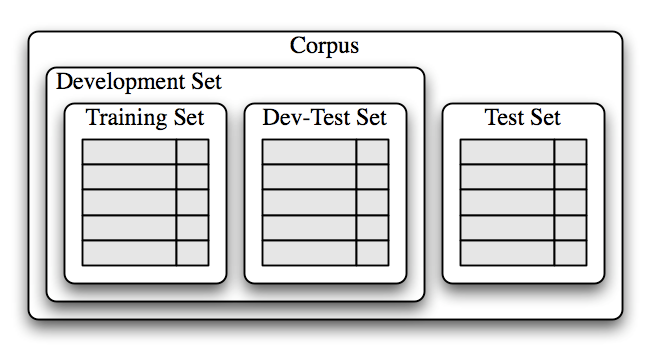
\includegraphics[width=0.8\textwidth]{Corpus.png}
\end{center}

\subsection{The statistic}

There are two different methods to process language problem. One is building the system by rules, another is based on statistic.

If we implement our system based on rules. First step is performing lexical analyst, then parser the sentence and analyst syntax, after execute semantic parsing, the last is context analyst. So if we would like to predict the form, the processing is inverse. 

For example, we need to predict form of the word 'become' in our sentence which contains by lemmas: "a standardized version of the game eventually become know as bagatelle."
First we need to know the grammatical tense according to the context, if it's past tense, then we analyst semantic meaning, then parser and perform lexical analysis, at last we should know the form of the word 'become' is mapping to 'became'.

Another method is by mathematic statistical processing. We build the mathematic model to learn the feature or rule for the problem. We can choose different statistic methods like Naive Bayes, HMM, or machine learning to train our model. By using statistic method, we calculate the probability of the form by the model, then we choose the highest probability as the predict result. 

\subsection{Reduce the noise}
Noise is an unavoidable problem, and it is the first step we have to deal with them. Because it will affect the data preparation processes in our development and cause errors due to the predict result less accurate.
Analyst the data and we found that there is one kind of noise in them. We think they may introduced by encoding problem. When the data is encoded by utf-8, after decoding them, there is lots of messy meta in these data. \todo{Please explain the solution on this problem}

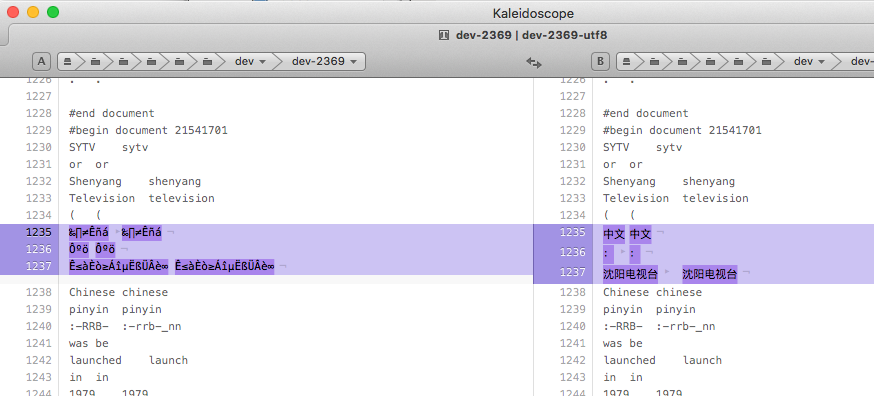
\includegraphics[width=1\textwidth]{noise1.png}

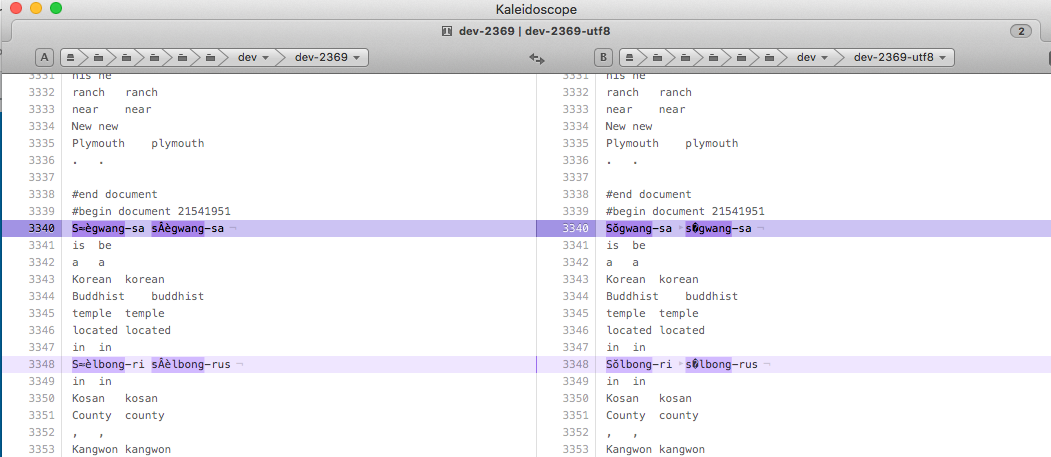
\includegraphics[width=1\textwidth]{noise2.png}

\subsection{Baseline}
Si on faisait rien, combien de précision de prédiction a-t-on gagné? \todo{Not sure if we still need to keep this part}

\section{Tool to implement our idea}
\subsection{Traitement}
There are some open source tools for handling Natural Language process, we compared some of them and finally decided to use NLTK in Python because of the program language and the mathematic statistic models it contains. 
We list some features of these open source tools for the future needs in case:
\href{https://stanfordnlp.github.io/CoreNLP/}{Stanford\'s CoreNLP:} linguistic analysis tools, Java
\href{http://textblob.readthedocs.io/en/dev/}{TextBlob:} Word inflection and lemmatization, Java
NLTK: Naive Bayes, HMM, N-gram Tagger + Python
\href{SpaCy: 13 statistical models, deep learning + Python
Apache Lucene and Solr
Apache OpenNLP
GATE and Apache UIMA 
Gensim

CST's lemmatiser: base on Brills rules (C++)
MorphAdorner: multi (Java)
Specialist NLP Tools Norm:dTagger (Java)
Stanford CoreNLP:ME (Java)
NLTK: base on HMM, Trigram Tagger、N-gram Tagger (Python)
SpaCy: (Python)

\subsubsection{Comparison parmi NLTK, TextBlob, Stanford CoreNLP, SpaCy and Gensim}
\begin{itemize}
\item Modèles entraîné ou pas?
\item La vitesse
\item NLTK vs. spaCy  Selon https://blog.thedataincubator.com/2016/04/nltk-vs-spacy-natural-language-processing-in-python/, spaCy est 20 fois plus vite que NLTK sur le travail de POS.
\end{itemize}
\subsubsection{NLTK}
\begin{enumerate}
\item Il faut considérer que les donnée on va nourrir au NLTK est dans quelle forme. En fait, nous sommes distribué les donnés dans la paire de frome-lemma.
\end{enumerate}

\subsection{Evaluation}
\begin{itemize}
\item Shell
\item Python
\item Excel
\end{itemize}

\section{Fondations de l’Algorithme}
\subsection{N-gram model}
Je ne veut pas enlever la ponctuation maintenant. Comme je crois que ils aident la prédiction.  Par example:
- bigram = ('', 'the')       The : the    =  19142.1 : 1.0
Si le mot avant "the" est ""(blank), puis "the" sera "The" avec t en majuscule. Parce que c'est normalement le debut d'une phrase.

These words are not independent, if we need to consider all the hypotaxis between these words, we consider to use Markov model to get the probability for the sentence: $P(s)=\prod\limits_{i=1}^{n}P(w_i|w_1...w_{i-1})$

\href{https://en.wikipedia.org/wiki/Markov_chain}{Markov chain}: A Markov chain is "a stochastic model describing a sequence of possible events in which the probability of each event depends only on the state attained in the previous event."

An n-gram model is an expended Markov model, for our case, it means the form for current word, it depends by previous n words. if n = 1, then the form depends by previous word, if n = 2, it's depends by previous 2 words, if n-gram, then we use this one to get the probability for the sentense: $P(s)=\prod\limits_{i=1}^{n}P(w_i|w_{i-n+1},...,w_{i-1})$

n = 1(unigram): $P(s)=\prod\limits_{i}P(w_i)$, e.g. $P(x_1,x_2,...,x_{10}) = P(x_1)P(x_2)...P(x_{10})$

n = 2(bigram): $P(s)=\prod\limits_{i}P(w_i|w_{i-1})$, e.g. $P(x_1,x_2,...,x_{10}) = P(x_1)P(x_2|x_1)P(x_3|x_2)...P(x_{10}|x_9)$

For our case, we predict the sentense, for example: 
s = "Year 208 BC was a year of the pre-Julian Roman calendar." 
That is P(s) = P(Year)P(208|Year)P(BC|208)...P(calendar|Roman)P(.|calendar)

So N-gram helps to predict the sentence.

NLTK:
\begin{lstlisting}
class nltk.model.ngram.NgramModel(n, train, pad_left=True, pad_right=False, estimator=None, *estimator_args, **estimator_kwargs)[source]
\end{lstlisting}

\subsection{Naive Bayes}
Naive Bayes is a classification technique based on Bayes' theorem with independence assumption.  given a problem instance to be classified, represented by a vector ${\mathbf  {x}}=(x_{1},\dots ,x_{n})$ representing some n features (independent variables), it assigns to this instance probabilities for each of K possible outcomes or classes $C_{k}$. \cite{murty_pattern_2011}

\[p(C_{k}\mid x_{1},\dots ,x_{n})={\frac {1}{Z}}p(C_{k})\prod _{i=1}^{n}p(x_{i}\mid C_{k})\]

With the the "naive" conditional independence assume that each feature $x_{i}$ is conditionally independent of every other feature $x_{j}$ for $j \neq i$, given the category. 

The prediction lemma-form problem, For Any given lemma $l_i$ we suppose that there is a form list $Forms(l_i)=\{f_{i1},f_{i2},...,f_{ik}\}$ which contains all its possible forms. The lemmas sequence $(l_1,l_2,...,l_n)$ are the sequence we can observe, so we take them as features. Then the form sequence is the classes that we want to put the features in\footnote{We will probably use both "label" or "class","tag" or "classify" in this notes, they will mean same thing.}. Actually,in this way,  we built up a label list contains all the forms show up in the corpus $\{Forms(l_1),Forms(l_2),..., Forms(l_n)\}$, the size of this list will be $V$, which is the total vocabulary of the forms in the corpus. Unfortunately, due to the immense of the vocabulary, the conditional probabilities table will be infeasible.

\[p(V|l_1,...,l_n) = \frac{1}{Z} p(V) \prod _{i=1}^{n}p(l_i \mid V) \]

Actually when we do predicting for the lemma $l_i$ in a sequence $(l_1,l_2,...,l_n)$, we just need to look at $Forms(l_i)$ and don't have to take account the $Forms(l_j)$ ($j \neq i$). In this section, We see the prediction of form for each lemma $l_i  \Longrightarrow f_i$ as a classification by choosing the labels only from $Forms(l_i)$. It's reasonable since the lemma is kind of the product of the lemmalization of the correspond forms $\{f_{i1},f_{i2},...,f_{ik}\}$. The one feature NB model correspond to our problem is like:

\[p(f_i|l_i) \propto p(f_i) \cdot  p(l_i|f_i)\]

Thus we apply the Naive Bayes Model to our lemma-form prediction. Express our idea using Bayesian probability terminology:\todo{If the essay is too long, delete here.}

\begin{align*}
posterior  &= \frac{prior \times likelihood}{evidence} \\
           &\propto  prior \times likelihood \\
\end{align*}
When we compare the probability of different form for lemma $l_i$, we are comparing the $p(f_i|l_i)$, posteriors  of lemma $l_i$ predicted as form $f_i$. It depends on the prior of the form $f_i$ and the likelihood of the lemma $l_i$ when form $f_i$ shows.
\begin{equation}
\frac{p(f_i|l_i)}{p(f_j|l_i)} = \frac{p(f_i) \cdot p(l_i \mid f_i)}{  p(f_j) \cdot p(l_i \mid f_j) } \qquad \qquad  f_i,f_j \in Forms(l_i)
\end{equation}
And $p(f_i) \cdot p(l_i \mid f_i)$ can even be simplified if we apply the MLE estimator $\frac{f}{n}$ to it.
\begin{equation} 
\label{eq:simple_mle}
\begin{aligned}
\hat{p}(f_i) \cdot \hat{p}(l_i \mid f_i) &= \frac{freq(f_i)}{n} \cdot \frac{freq(l_i, f_i)}{freq(f_i)} \\
&= \frac{freq(l_i, f_i)}{n}
\end{aligned}
\end{equation}

The equation \ref{eq:simple_mle} is a simple theoretical model. It maybe a little astonishing that,based on this model, if we want to compare $p(f_i|l_i)$ and $p(f_j|l_i)$, just need to compare the co-occurrence $freq(l_i,f_i)$ and $freq(l_i,f_j)$.  The problem is we can't deal with those lemmas we haven't seen. Since we use NLTK package, the smooth method of NLTK will be given later on. 

And since one time training will prepare the parameters for the prediction for one lemma, if the train set contains $n$ different lemmas, then the model will be trained $n$ times. Nevertheless the same lemma will share the same parameters. So we use a dictionary to store them to avoid the the repetition work.


\todo{Should be moved after the smooth part}
Take the lemma "find" in file <dev-24> as an example. The first 90\% of the file is taken as the train set (N=1576467). Table \ref{tb:cfd_find} shows the conditional frequency of the forms of "find" in the train set. It means $freq(lemma="find", form="found")=778$, $freq(lemma="find",form="find")=204$ etc.

\begin{table}[htb]
\centering
\begin{tabular}{|l|llllll|}
\hline
form $f_i$       & found & find & finds & finding & Finding & Finds \\ \hline
freq($f_i$,"find") & 778   & 204  & 65    & 32      & 4       & 2     \\ \hline
freq($f_i$) & 778   & 204  & 65    & 45      & 4       & 2     \\ \hline
\end{tabular}
\caption{conditional frequency of the forms of "find"}
\label{tb:cfd_find}
\end{table}

Although we don't even need to use the $freq(f_i)$ in our current model, it's for the future use.

Suppose our one feature NB model is classifying the lemma "find", the only feature is \{"lemma":"find"\}\footnote{In fact, the final format of feature we use is \{"find":True\}} and the classes to be chosen from are \{found, find, finds, finding, Finding, Finds\}. The model will compare the max $p(f_i|l_i)$ and do the classification. No doubt, $p("found" | lemma="find")$ is the max, thus the classes will always be form "found". We call this unigram. Because this model just has one feature and only the $l_i$ will affect the classes $f_i$. 

The bigram model we built is taking account the influence of the $l_{i-1}$ to $f_i$.
\begin{align}
p(f_i|l_{i-1},l_i) &\propto p(f_i) \cdot  p(l_{i-1},l_i|f_i)  \\
&= p(f_i) \cdot  p(l_{i-1}|f_i) \cdot p( l_i | l_{i-1},f_i) \label{eq:bigram_mod} \\
&= p(f_i) \cdot  p(l_{i-1}|f_i) \cdot p( l_i | f_i) \label{eq:bigram_nb}
\end{align}

Apply the Naive Bayes assumption to get from equation \ref{eq:bigram_mod} to \ref{eq:bigram_nb}. And in our case, if we see "to find" to the probability of classifying "find" into "finding"   it would be:
\begin{equation}
p(finding | to,find) \propto p(finding)\cdot p(to | finding) \cdot  p(find | finding))
\end{equation}
$"finding":form_i \quad "to":lemma_{i-1} \quad "find":lemma_i$


We face the problem then, how can we prepare the feature set to feed the NLTK Naive Bayes model? The feature is \{"lemma-1":"to","lemma":"find" \} or 
 \{"bigram":("to","find"),"lemma":"find" \}? Or both of them are incorrect? 
\subsubsection{Smooth method of NLTK Naive Bayes}
The euation 2 already does its job. But it has a fatal problem. It can't tackle the un-seen lemmas. 

According to the source code of NLTK class NaiveBayesClassifier, it takes Expected Likelihood Estimate method, the probability distribution is given as below:
\begin{equation}
p(x_i)=\frac{C+0.5}{N+B/2} \qquad X = \{x_1,x_2,\dots,x_o,\dots\}
\end{equation}

$C$ is the frequency we count with $N$ outcomes and $B$ the number of the observed value of $X$. As addressed in the comment of the source code:\footnote{\url{http://www.nltk.org/_modules/nltk/probability.html}}
\begin{quotation}
This is equivalent to adding 0.5 to the count for each bin, and taking the maximum likelihood estimate of the resulting frequency distribution.
\end{quotation}

\todo{Compare the ELE and MLE}

\subsubsection{Feature format}


Additionally, we assume that for two lemmas $l_i$ and $l_{i+1}$, the prediction form $f_{i}$ is independent of every other $f_{j}$ for $j \neq i$. Obviously, it's not realistic. For example, the lemma series "student be", if the "student" is predicted as "students", then the "be" should be either "are" or "were". 



\textcolor{red}{How to use smoothing?}
{ Nos variables aléatoires sont discrètes. -> MultiNomial Naive Bayes -> Smoothing}

\textcolor{red}{Is that possible overfit if using Naive Bayes?}

\subsection{Modèles de Markov cachée HMM}
\begin{itemize}
\item Théorie

The HMM is an extension to the Markov chain.



A HMM can be characterised by:
\begin{itemize}
\item the output observation alphabet. This is the set of symbols which may be observed as output of the system.
\item the set of states.
\item the transition probabilities $a_{ij} = P(s_t = j | s_{t-1} = i)$. These represent the probability of transition to each state from a given state.
\item the output probability matrix $b_i(k) = P(X_t = o_k | s_t = i)$. These represent the probability of observing each symbol in a given state.
\item the initial state distribution. This gives the probability of starting in each state.
\end{itemize}

The output observation alphabet is the set of word forms (the lexicon), and the 
remaining three parameters are derived by a training regime.

HMM regards to the optimal combination of tags for a larger unit, such as a sentence.

Viterbi algorithm, which efficiently computes the optimal path through the graph given the sequence of words forms.

The most difficult task with the model, and requires either MLE estimates of the parameters or unsupervised learning using the Baum-Welch algorithm, a variant of EM.


\item Lier les séquences aux états
\item Lissage
\item Apprentissage des paramètres
\end{itemize}


\subsection{Générateur vs Discriminant}

\subsection{Local Maximum}

\subsection{Label bias problem}

\section{Related work}
Compare
\begin{lstlisting}
labeled_features_1a = [({"lemma":"the"},'the'), ({"lemma":'be'},'is'), ({"lemma":'be'},'is'), ({"lemma":'be'},'was')]
labeled_features_1b = [({'the':True},'the'), ({'be':True},'is'), ({'be':True},'is'), ({'be':True},'was')]
\end{lstlisting}

\begin{lstlisting}
labeled_features_2a = [({"lemma":"do"},'do'), ({"lemma":"the"},'the'), ({"lemma":'be'},'is'), ({"lemma":'be'},'is'), ({"lemma":'be'},'was')]
labeled_features_2b = [({'do':True},'do'), ({'the':True},'the'), ({'be':True},'is'), ({'be':True},'is'), ({'be':True},'was')]
\end{lstlisting}

\section{Discussion}
\section{Résumé}
\cite{greenwade93}


\bibliographystyle{apacite}
\bibliography{jason,sample}
\end{document}